\documentclass[
    oneside,
    fontsize=13pt,          % default font size 12pt
    paper=a4,               % DIN A4 page format
    numbers=noenddot,       % remove dots behind chapter numbers (e.g. 1.5 not 1.5.)
    listof=totoc,           % add list of figures, tables, etc. to ToC
    listof=entryprefix,     % add entry name to figures, tables, etc.
    listof=nochaptergap,    % no chapter gap for figures, tables, etc.
    bibliography=totoc,     % add bibliography to ToC but without a chapter number
    % parskip=half            % half line spacing between paragraphs
]{scrbook}

% ##################################################
% ENCODING
% ##################################################
\usepackage{cmap}               % PDF character encoding
\usepackage[T1]{fontenc}        % 8-bit font encoding
\usepackage[utf8]{inputenc}     % UTF-8 input encoding
\usepackage{caption}
\usepackage{subcaption}

% ##################################################
% DOCUMENT VARIABLES
% ##################################################
% Personal data
\newcommand{\docAuthor}{Simeon Messerschmidt, ...}
\newcommand{\docMatriculationNumber}{260322}
\newcommand{\docStudyProgram}{Allgemeine Informatik}
\newcommand{\docStreetName}{Straße}
\newcommand{\docPostalCode}{PLZ}
\newcommand{\docCity}{Furtwangen}
\newcommand{\docEmail}{mail}

% Document data
\newcommand{\docTitle}{Projekt Dokumentantion}
\newcommand{\docSubTitle}{Out of Band Provisioning for IOT devices} 
% \newcommand{\docType}{Bachelor Thesis}
\newcommand{\docSupervisor}{Prof...}
\newcommand{\docCoSupervisor}{Betreuuer ...}
\newcommand{\docDeadline}{05.10.2022}


% ##################################################
% GENERAL
% ##################################################
\usepackage{scrhack}            % better KOMA adaptions
\usepackage[table]{xcolor}      % color support
\usepackage{chngcntr}           % for renumbering stuff


% ##################################################
% PDF SETTINGS
% ##################################################
\usepackage[
    colorlinks=false,
   	linkcolor=black,
   	citecolor=black,
  	filecolor=black,
	urlcolor=black,
    bookmarks=true,
    bookmarksopen=true,
    bookmarksopenlevel=3,
    bookmarksnumbered,
    plainpages=false,
    pdfpagelabels=true,
    hyperfootnotes,
    pdftitle ={\docTitle},
    pdfauthor={\docAuthor},
    pdfcreator={\docAuthor}
]{hyperref}


% ##################################################
% FONTS AND SPACING
% ##################################################
\renewcommand{\familydefault}{\sfdefault}   % default font
\usepackage[onehalfspacing]{setspace}       % default 1.5 spacing
\raggedbottom   % don't stretch spacing to fit page length

% font sizes and styles
\addtokomafont{chapter}{\sffamily\large\bfseries} 
\addtokomafont{section}{\sffamily\normalsize\bfseries} 
\addtokomafont{subsection}{\sffamily\normalsize\mdseries}
\addtokomafont{caption}{\sffamily\normalsize\mdseries}

% url font style
\usepackage{relsize}
\renewcommand*{\UrlFont}{\ttfamily\smaller\relax}


% ##################################################
% PAGE FORMATTING
% ##################################################
% Page layout
\usepackage[
	bindingoffset=1.5cm,
	inner=2.5cm,
	outer=2.5cm,
	top=3cm,
	bottom=2cm
]{geometry}

% Page header
\usepackage[
    headsepline,        % seperator line beneath page header on normal pages
    plainheadsepline    % seperator line beneath page header on pages like ToC
]{scrlayer-scrpage}
\clearpairofpagestyles                  % clear default settings
\addtokomafont{pagehead}{\normalfont}   % use normal font for page header
\ohead*{\thepage}                       % page number
\ihead*{\leftmark}                      % chapter name


% ##################################################
% IMAGES AND FIGURES
% ##################################################
\usepackage{graphicx}       % support for including images
\graphicspath{{pictures/}}  % default path

% simple numbering without chapter
\renewcommand{\thefigure}{\arabic{Abbildung}}
\counterwithout{figure}{chapter}

% ##################################################
% TABLES
% ##################################################
\usepackage{booktabs}   % beautiful table style
\usepackage{multirow}   % multi row and multi column table functionality

% simple numbering without chapter
\renewcommand{\thetable}{\arabic{table}}
\counterwithout{table}{chapter}

% ##################################################
% SOURCE CODE LISTINGS
% ##################################################
\usepackage{listings}
\usepackage{beramono}   % use a typewriter font which supports bold characters

\renewcommand{\lstlistlistingname}{List of Code Listings}   % 
\renewcommand{\lstlistingname}{Code Listing}
\newcommand{\listoflolentryname}{\lstlistingname}   % prefix for List of Code Listings

% define colors for source code highlighting
\definecolor{codegreen}{rgb}{0,0.6,0}
\definecolor{codegray}{rgb}{0.5,0.5,0.5}
\definecolor{codepurple}{rgb}{0.5,0,0.33}
\definecolor{codepurblue}{rgb}{0.16,0.0,1.0}
\definecolor{backcolour}{rgb}{0.95,0.95,0.92}

% set source code style
\lstdefinestyle{codestyle}{
    backgroundcolor=\color{backcolour},   
    commentstyle=\color{codegreen},
    keywordstyle=\bfseries\color{codepurple},
    numberstyle=\tiny\color{codegray},
    stringstyle=\color{codepurblue},
    basicstyle=\scriptsize\ttfamily,
    breakatwhitespace=false,
    breaklines=true,
    captionpos=b,
    keepspaces=true,
    numbers=left,
    numbersep=5pt,
    showspaces=false,
    showstringspaces=false,
    showtabs=false,
    tabsize=2,
    escapeinside={(*@}{@*)}
}
\lstset{style=codestyle, numberbychapter=false}


% ##################################################
% TABLE OF CONTENTS
% ##################################################
\KOMAoptions{toc=chapterentrydotfill}       % dotted lines for chapters
\addtokomafont{chapterentry}{\normalfont}   % use normal font for chapter entries

% spacing
\DeclareTOCStyleEntry[beforeskip=0cm]{chapter}{chapter}
\DeclareTOCStyleEntry[beforeskip=0cm]{section}{section}
\DeclareTOCStyleEntry[beforeskip=0cm]{default}{subsection}

% colons after entry names
\BeforeStartingTOC[lof]{\def\autodot{:}}
\BeforeStartingTOC[lot]{\def\autodot{:}}
\BeforeStartingTOC[lol]{\def\autodot{:}}


% ##################################################
% BIBLIOGRAPHY
% ##################################################
\usepackage{csquotes}
\usepackage[backend=biber,citestyle=ieee]{biblatex}
\addbibresource{bibtex.bib}
\setlength\bibitemsep{.5\baselineskip}
\setcounter{biburlnumpenalty}{9000} % break URLs on numbers
\setcounter{biburllcpenalty}{9000}  % break URLs on lower case letters
\setcounter{biburlucpenalty}{9000}  % break URLs on upper case letters


% ##################################################
% ABBREVIATIONS
% ##################################################
\usepackage[printonlyused]{acronym}


% ##################################################
% APPENDIX
% ##################################################
\usepackage[title,titletoc]{appendix}

% appendix chapter
\newcommand{\appendixchapter}[1]{
   \cleardoublepage
    \pagenumbering{arabic}
    \renewcommand{\thepage}{\thechapter-\arabic{page}}
    \chapter{#1}
}

% insert monthly report pdf as picture in order to keep page header
\newcommand{\monthlyreport}[2]{
    \section{#1}
    \centering
    \includegraphics[trim=55 35 55 35,clip,width=1\textwidth]{#2}
    \clearpage
}


% ##################################################
% MISC
% ##################################################
% better referencing of images, tables, etc.
\usepackage[nameinlink, noabbrev]{cleveref}                       % load preamble

\begin{document}

\begin{titlepage}
\pagestyle{empty}

% HFU Logo
\begin{flushright}
    \begin{figure}[ht]
        \flushright
        
\includegraphics[height=2cm]{pictures/hfu_logo_vector_4C.eps}
    \end{figure}
\end{flushright}

\begin{center}
    % {\fontsize{18}{22} \selectfont \docType}\\[5mm]
     % {\fontsize{18}{22} \selectfont in the field of} \\[5mm]
    {\fontsize{18}{22} \selectfont \docStudyProgram}\\
    
    \vspace{1cm}
    
    {\fontsize{22}{26} \selectfont \textbf{\docTitle}}\\[5mm]
    {\fontsize{18}{22} \selectfont \docSubTitle}

    \vspace{6cm}
    
    \begin{tabular}{ll}
        Ansprechspartner:   & \docSupervisor    \\\\
        Betreuer:           & \docCoSupervisor  \\\\   
        submitted on:       & \docDeadline      \\\\
        submitted by:       & \docAuthor        \\
                            & matriculation~number:~\docMatriculationNumber\\
                            & \docStreetName,~\docPostalCode~\docCity\\
                            & \docEmail         
    \end{tabular}
\end{center}
\end{titlepage}           % title page

% Roman numbering
\frontmatter
\pagenumbering{Roman}

% \include{framework/einleitung}
\renewcommand*\contentsname{Inhaltsverzeichnis}            % Abstract
\tableofcontents                                            % Contents
\renewcommand{\figurename}{Abbildung}
\renewcommand{\bibname}{Quellenverzeichnis}

% Content
\mainmatter
\chapter{Einleitung}

%\section{How to Use This Document}
%This document has been designed to be used with Overleaf. However, you should be able to compile it with any LaTeX environment. In case you have never worked with LaTeX before, it may be a good idea to do some tutorials first. The Overleaf documentation explains all important LaTeX concepts and contains helpful examples for all kinds of stuff: \url{https://www.overleaf.com/learn/latex/Main_Page}\par

%Unfortunately, \acl{HFU} does not provide an official LaTeX thesis template at this point in time. This template is student-made and therefore unofficial. Although it has been designed to follow all required guidelines, you should probably double check everything in case these guidelines changed. Use this at your own risk.\par

%In the following, we explain some basic functionality regarding this template.

%\section{Abbreviations}
%Abbreviations can be defined in the abbreviations.tex file. Once you defined them, you can use them in a sentence like this: \ac{HFU}. As you can see, the first occurrence of an abbreviation will be inserted as a non-abbreviated version followed by the abbreviation in brackets. If you use this abbreviation again, it won't insert the non-abbreviated form anymore: \ac{HFU}. However, you can force different versions at any point: for the short version use \acs{HFU}, for the long version use \acl{HFU} and for the full version use \acf{HFU}. Additionally, you can print the plural of an abbreviation (although it doesn't make any sense in this case) using \acsp{HFU}. 

%\section{Citations}
%itations are implemented using BibLaTeX and will be displayed in IEEE style. Add your bibtex entries to the bibtex.bib file. After that, you can cite them as shown in the following examples.

%\subsection{Normal Quote}
%This is a normal sentence but we used an external source to come up with its content. Therefore, we must cite the external source using a reference like this: \cite{example}

%\subsection{Direct Quote}
%\begin{quote}
 %   \textit{\enquote{This is a direct quote. Direct quotes are displayed using quotation marks and must be copied word by word from the original source.}} \cite{example}
%\end{quote}

%\subsection{Refering to Content Within This Document}
%\label{example_label}
%You can add a label mark at any position on the page as well as figures, tables and code listings. Exemplary, we labeled this subsection and can refer to it like %this:  \cref{example_label}. You can also use \Cref{example_label}, if you want to capitalize the reference at the start of a sentence.


%\section{Figures}

%Figures can be inserted as shown below. Check out the Overleaf documentation for more information on how to use and style figures to your liking: \url{https://www.overleaf.com/learn/latex/Inserting_Images} As already mentioned above, you can refer to figures by citing its label: \cref{pic:hfu_logo} or \Cref{pic:hfu_logo}
%\begin{figure}[ht]  % figure position
 %   \centering      % center the image
%    
\includegraphics[width=.5\textwidth]{hfu_logo_vector_4C.eps}
%    \caption{HFU Logo}      % caption the image
 %   \label{pic:hfu_logo}    % label the image for internal referencing
%\end{figure}


%\section{Tables}

%Tables can be inserted as shown below. Check out the Overleaf documentation for more information on how to use and style tables to your liking: \url{https://www.overleaf.com/learn/latex/Tables}

%\begin{table}[ht]   % table position
   % \centering
  %  \footnotesize
  %  \begin{tabular}{lcr} % columns and their alignment
   %     \toprule    % separator line
  %      Left-aligned column  & Centered column  & Right-aligned column \\
  %      \midrule    % separator line
  %      Value 1 & Value 2 & Value 3 \\
 %       Value 4 & Value 5 & Value 6 \\
  %      Value 7 & Value 8 & Value 9 \\
  %      \bottomrule % separator line
  %  \end{tabular}
  %  \caption{Example table}
  %  \label{table:example_table}
%\end{table}


%\section{Source Code Snippets}
%Source code can be inserted as shown below. Syntax highlighting is supported for many popular languages. As always, we can define a caption and a label to %reference like this: \cref{code:helloworld} or \Cref{code:helloworld}

%\begin{lstlisting}[language=Java, caption=Hello World in Java, label=code:helloworld]
%public static void main(String args[]){
%    System.out.println("Hello World!");
%}
%\end{lstlisting}


%\section{That's it!}
%Congratulations! You know the basics of Latex as well as how to use this template and you are ready to start writing your thesis now. You can contribute to this template on GitHub in case you find any errors or add functionality.\par

%Good luck!
\chapter{Out of Band Provisioning for IOT devices}
    
\section{Kapitel}
\subsection{Sub Kapitel}
Beispiel Quellverlinkung \cite{[1]}
%

Einfügen von Bildern
\begin{figure}[h]
    \centering
    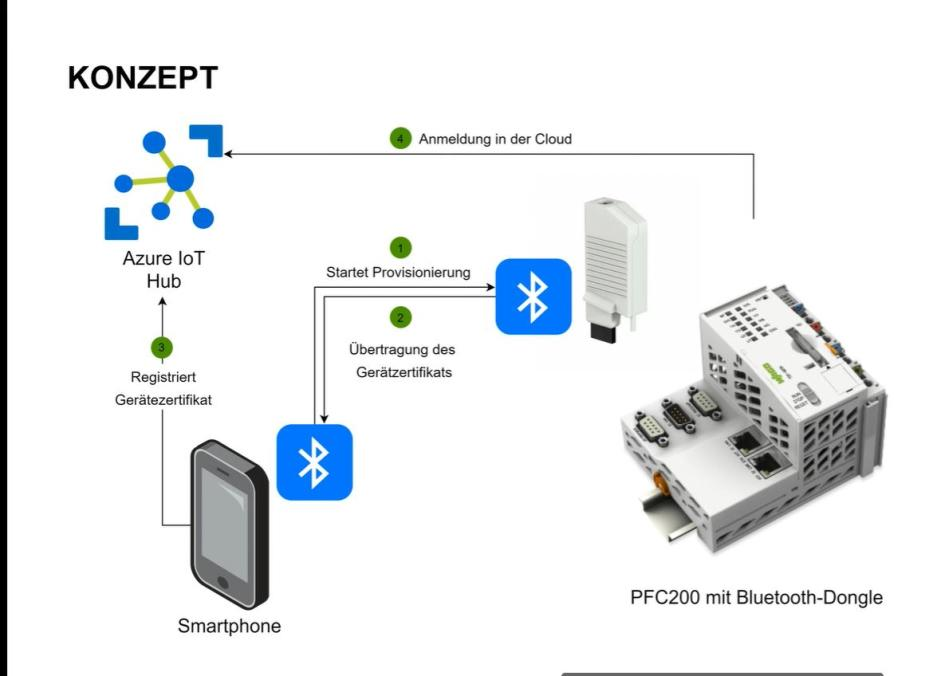
\includegraphics[width=15cm]{pictures/entwurf}
    \caption{Aktivitäts Diagramm}
\end{figure}

\chapter{Kritische Bewertung und Reflexion}

Reflexion








\chapter{Zusammenfassung und Fazit}

conclusion


\renewcommand{\listfigurename}{Abbildungsverzeichnis}
\listoffigures                          % List of Figures
%\listoftables                           % List of Tables
%\lstlistoflistings                      % List of Code Listings
%\include{framework/abbreviat{UndNochEinZitat}ions}       % Abbreviations
% \chapter*{Quellenverzeichnis\markboth{Quellenverzeichnis}}

\begin{thebibliography}{999}
\bibitem{[1]} \url{https://mediapipe.dev/}
\bibitem{trello} \url{https://trello.com/}
\end{thebibliography}


\begin{thebibliography}{999}
\bibitem{[1]}{Mediapipe: }\url{https://mediapipe.dev/}
\bibitem{[2]}{Trello: }\url{https://trello.com/}
\end{thebibliography}


% Bibliography
\begin{singlespace}
    \printbibliography
\end{singlespace}

% Declaration of Authorship (in German)
\chapter*{Eidesstattliche Erklärung\markboth{Eidesstattliche Erklärung}{}}
\addcontentsline{toc}{chapter}{Eidesstattliche Erklärung}
Ich versichere, dass ich die vorstehende Arbeit selbstständig verfasst und hierzu keine anderen als die angegebenen Hilfsmittel verwendet habe. Alle Stellen der Arbeit die wörtlich oder sinngemäß aus fremden Quellen entnommen wurden, sind als solche kenntlich gemacht.
\\ \\
Die Arbeit wurde bisher in gleicher oder ähnlicher Form in keinem anderen Studiengang als Prüfungsleistung vorgelegt oder an anderer Stelle veröffentlicht.
\\ \\
Ich bin mir bewusst, dass eine falsche Erklärung rechtliche Folgen haben kann.

\vspace*{1.5cm} \par
\line(1,0){200} \par
\docCity, \docDeadline ~~\docAuthor
   


\end{document}
